% Drawing 154/02-13 -- folder 154, batch 02, archive page 38 (PDF page 39).
% Transcription: figure : deux disques au bord vert traversés de cordes orange, régions voisines du bord coloriées en jaune ; sur chacun, les extrémités $u$, $v$ en haut (une flèche au-dessus), et deux cordes $D$, $D'$ ; « $+$ » entre eux, puis « $=$ » et une accolade qui renvoie à un troisième disque accolé au premier par le bas, les extrémités $s$, $t$ et $t$, $s$ se touchant au point de contact, de petites flèches courbes marquant l'échange des extrémités, et en bas $v$, $u$
% Kind: sum of two chord systems in disks, glued result. Method 2 (schematic redraw from the facsimile). Status: partial.
% Notes: Two disks with green rims crossed by orange chords, regions by the rim coloured (drawn as small orange wedges); on each the ends u, v at the top (an arrow above the first), and two chords D, D'; « + » between them, then « = » and a curved stroke sending to a third disk glued under the first, the ends s, t and t, s touching at the contact, and v, u at the bottom; the small curved arrows of the exchange are left out. Read from the page view; chords schematic.
% Coordinates: 1 unit = 1 mm = 1/100 of the crop width (bbox in page fractions: [0.175, 0.159, 0.402, 0.271]).
% Redrawn by Claude (claude-opus-5-5), issue #73, 2026-11-07; not checked by a human; not compiled (no TeX in the session).
% Rights: reproduces part of the work -- behind RENDER_TRANSCRIPTS, never published by itself.
\documentclass[tikz,border=3pt]{standalone}
\usepackage{amsmath,amssymb}
\usetikzlibrary{patterns,arrows.meta}
\tikzset{Or/.style={orange!90!black}, Ye/.style={yellow!80!orange}, Lg/.style={green!60!black!70}, Dg/.style={green!45!black}, Br/.style={brown!80!black}, Rd/.style={red!85!black}, Bl/.style={blue!70!black}, Gy/.style={black!40}, pencil/.style={black!45}, struck/.style={black!35}, mark/.style={circle,draw,inner sep=1.3pt}, pt/.style={circle,fill,inner sep=0.9pt}, opt/.style={circle,draw,fill=white,inner sep=1.1pt}}
\begin{document}
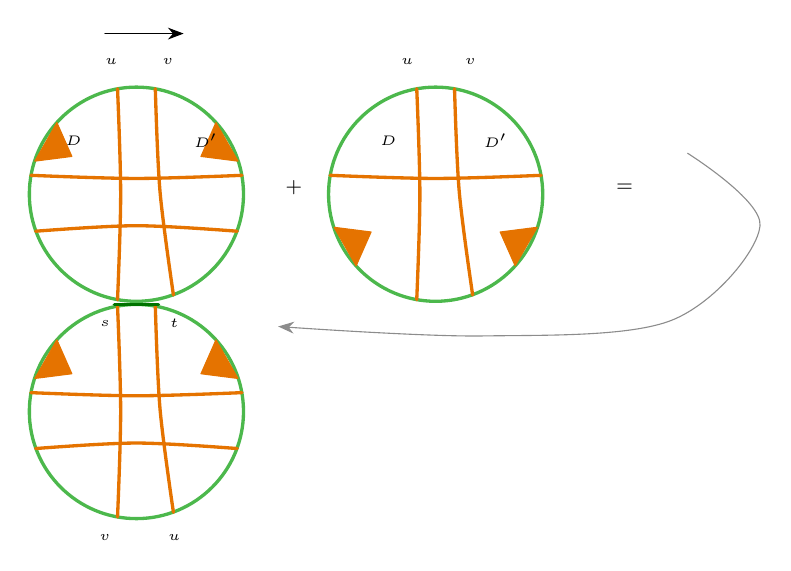
\begin{tikzpicture}[x=1mm,y=1mm,line cap=round,line join=round,font=\scriptsize]
\draw[Lg,very thick] (16,-24) ellipse[x radius=13.6, y radius=13.6];
\draw[Or,very thick] plot[smooth, tension=0.55] coordinates {(13.6,-10.6) (14,-24) (13.6,-37.4)};
\draw[Or,very thick] plot[smooth, tension=0.55] coordinates {(18.4,-10.6) (19,-23.7) (20.7,-36.8)};
\draw[Or,very thick] plot[smooth, tension=0.55] coordinates {(2.6,-21.6) (16,-22) (29.4,-21.6)};
\draw[Or,very thick] plot[smooth, tension=0.55] coordinates {(3.2,-28.7) (16,-28) (28.8,-28.7)};
\draw[Or] (5.9,-14.9) -- (3.1,-19.8) -- (7.8,-19.2) -- cycle;
\fill[pattern=north east lines,Or] (5.9,-14.9) -- (3.1,-19.8) -- (7.8,-19.2) -- cycle;
\draw[Or] (28.9,-19.8) -- (26.1,-14.9) -- (24.2,-19.2) -- cycle;
\fill[pattern=north east lines,Or] (28.9,-19.8) -- (26.1,-14.9) -- (24.2,-19.2) -- cycle;
\node[inner sep=1pt] at (12.8,-7.2) {\tiny $u$};
\node[inner sep=1pt] at (20,-7.2) {\tiny $v$};
\draw[-{Stealth[length=2mm]}] (12,-3.6) -- (22,-3.6);
\node[inner sep=1pt] at (8,-17.2) {\tiny $D$};
\node[inner sep=1pt] at (24.8,-17.2) {\tiny $D'$};
\node[inner sep=1pt] at (12,-40.4) {\tiny $s$};
\node[inner sep=1pt] at (20.8,-40.4) {\tiny $t$};
\node[inner sep=1pt] at (36,-23.2) {\scriptsize $+$};
\draw[Lg,very thick] (54,-24) ellipse[x radius=13.6, y radius=13.6];
\draw[Or,very thick] plot[smooth, tension=0.55] coordinates {(51.6,-10.6) (52,-24) (51.6,-37.4)};
\draw[Or,very thick] plot[smooth, tension=0.55] coordinates {(56.4,-10.6) (57,-23.7) (58.7,-36.8)};
\draw[Or,very thick] plot[smooth, tension=0.55] coordinates {(40.6,-21.6) (54,-22) (67.4,-21.6)};
\draw[Or] (41.1,-28.2) -- (43.9,-33.1) -- (45.8,-28.8) -- cycle;
\fill[pattern=north east lines,Or] (41.1,-28.2) -- (43.9,-33.1) -- (45.8,-28.8) -- cycle;
\draw[Or] (64.1,-33.1) -- (66.9,-28.2) -- (62.2,-28.8) -- cycle;
\fill[pattern=north east lines,Or] (64.1,-33.1) -- (66.9,-28.2) -- (62.2,-28.8) -- cycle;
\node[inner sep=1pt] at (50.4,-7.2) {\tiny $u$};
\node[inner sep=1pt] at (58.4,-7.2) {\tiny $v$};
\node[inner sep=1pt] at (48,-17.2) {\tiny $D$};
\node[inner sep=1pt] at (61.6,-17.2) {\tiny $D'$};
\node[inner sep=1pt] at (78,-23.2) {\scriptsize $=$};
\draw[pencil,-{Stealth[length=2mm]}] plot[smooth, tension=0.55] coordinates {(86,-18.8) (95.2,-28) (84,-40) (60,-42) (34,-40.8)};
\draw[Lg,very thick] (16,-51.6) ellipse[x radius=13.6, y radius=13.6];
\draw[Or,very thick] plot[smooth, tension=0.55] coordinates {(13.6,-38.2) (14,-51.6) (13.6,-65)};
\draw[Or,very thick] plot[smooth, tension=0.55] coordinates {(18.4,-38.2) (19,-51.3) (20.7,-64.4)};
\draw[Or,very thick] plot[smooth, tension=0.55] coordinates {(2.6,-49.2) (16,-49.6) (29.4,-49.2)};
\draw[Or,very thick] plot[smooth, tension=0.55] coordinates {(3.2,-56.3) (16,-55.6) (28.8,-56.3)};
\draw[Or] (5.9,-42.5) -- (3.1,-47.4) -- (7.8,-46.8) -- cycle;
\fill[pattern=north east lines,Or] (5.9,-42.5) -- (3.1,-47.4) -- (7.8,-46.8) -- cycle;
\draw[Or] (28.9,-47.4) -- (26.1,-42.5) -- (24.2,-46.8) -- cycle;
\fill[pattern=north east lines,Or] (28.9,-47.4) -- (26.1,-42.5) -- (24.2,-46.8) -- cycle;
\node[inner sep=1pt] at (12,-67.6) {\tiny $v$};
\node[inner sep=1pt] at (20.8,-67.6) {\tiny $u$};
\draw[Dg,very thick] (13.2,-38) -- (18.8,-38);
\end{tikzpicture}
\end{document}
